\documentclass[a4paper,11pt,twocolumn]{article}
\usepackage[utf8]{inputenc}
\usepackage{amsmath,amssymb,amsfonts}
\usepackage{graphicx}
\usepackage{listings}
\usepackage{xcolor}
\usepackage{hyperref}
\usepackage{geometry}
\geometry{margin=0.75in}
\usepackage{CJKutf8}
\usepackage{cite}

\hypersetup{
    colorlinks=true,
    linkcolor=blue,
    citecolor=blue,
    urlcolor=blue
}

\title{\textbf{マクスウェルの悪魔とランダウアー限界：\\理論物理モデルから環境発電実機までの17桁の隔たりと熱力学的厳密性}}
\author{今井 健吾\footnote{Maxwells Demon Project} \quad et al.}
\date{2026年10月5日}

\begin{document}
\begin{CJK*}{UTF8}{min}

\twocolumn[
  \begin{@twocolumnfalse}
    \maketitle
    \begin{abstract}
    情報熱力学における「マクスウェルの悪魔」と「ランダウアーの原理」について、理論モデルの熱力学的整合性の厳密な再検証と、ESP32-C3 マイクロコントローラを用いた自律型環境発電デモ装置（構成D）の実装・評価を行った。第一に、量子ドット3体系および10ドットチェーンのマスター方程式シミュレーションにおいて、局所 Lindblad 近似や演算子の割り当て誤りに起因する「見かけ上の第二法則突破（負の消去コストによる無限発電）」の物理的誤りを特定・補正し、等温環境下では正味仕事が常に非正 ($W_{\mathrm{net}} \le 0$) となる厳密な熱力学収支を示した。第二に、悪魔のメモリ消去部を極低温 ($4.2\text{ K}$) に配置する 2 温度構成、またはもつれ消費サイクルを考慮することで正味電力が得られる物理条件を整理した。第三に、体温熱電発電（TEG）駆動の ESP32-C3 自律給電実機において、制御ファームウェアの待機時間最適化（v2 ファームウェア）により起床中の消費エネルギーを $201\text{ mJ}$ から $0.79\text{ mJ}$ へ約 254 倍削減し、実機レベルでの正味エネルギー収支黒字化 ($W_{\mathrm{net}} > 0$) に成功した。さらに、理想的物理限界 ($k_B T \ln 2 \approx 2.87 \times 10^{-21}\text{ J}$) と実機コントローラの情報処理コスト ($0.66\text{ mJ}$) との間には約 $2.3 \times 10^{17}$ 倍の巨大な隔たりが存在することを定量化し、理論物理・数値シミュレーション・実用工学を結ぶ包括的な知見を提示する。
    \end{abstract}
    \vspace{1em}
    \begin{center}
      \small \textbf{キーワード}: マクスウェルの悪魔, 情報熱力学, ランダウアーの原理, 量子エンタングルメント, エントロピー生成, 環境発電, 深層強化学習
    \end{center}
    \vspace{1.5em}
  \end{@twocolumnfalse}
]

\section{緒論}
1867年に Maxwell が提唱した「マクスウェルの悪魔」\cite{maxwell1871theory} は、熱運動する分子の情報を観測して選別することで、外部から仕事を加えることなく温度差を生み出す思考実験である。Szilard (1929) \cite{szilard1929entropieverminderung} による情報とエントロピーの等価性の指摘を経て、Sagawa-Ueda 関係式 \cite{sagawa2008second} に代表される現代の情報熱力学では、獲得した相互情報量 $I$ を消費することで、等温環境下でも局所的に自由エネルギー以上の仕事 $W_{\mathrm{ext}} \le -\Delta F + k_B T \cdot I$ を抽出可能であることが証明されている。

しかし、悪魔が繰り返し動作して熱力学的サイクルを閉じるためには、獲得した情報を消去して初期状態に戻す必要がある。Landauer の原理 \cite{landauer1961irreversibility, bennett1982thermodynamics} によれば、1 ビットの不可逆な情報消去には最低でも $k_B T \ln 2$ の熱散逸が伴う。この消去コストの存在により、全体系（対象＋悪魔）としての正味の仕事抽出は不可能ですあり、熱力学第二法則は厳密に維持される。

近年、量子もつれ（エンタングルメント）を用いた「負の消去コスト」\cite{delrio2011thermodynamic} や、連続測定とベイズ推定に基づく情報エンジン \cite{koski2014experimental, strasberg2017quantum} が注目を集めている。しかし、数値シミュレーションや物理解釈において、演算子の定義ミスや局所 Lindblad 方程式の適用限界 \cite{levy2014local}、あるいは実機コントローラの消費電力と物理的ランダウアー限界の混同に起因して、「室温で第二法則を突破する第二種永久機関が成立した」という誤った結論が導入されるケースが散見される。

本論文では、量子ドット情報エンジンの数値モデルの熱力学的厳密性を再検証するとともに、理論極限と実機マイクロコントローラ（ESP32-C3）との間の定量的なエネルギーギャップを明示し、理論・シミュレーション・実機工学を正しく架橋する知見を報告する。

\section{量子情報エンジンモデルの熱力学的再検証}

\subsection{3重ドット自律デーモンとエントロピー生成率}
ワーキング物質となる2つの量子ドット ($L, R$) と、それらの占有状態を非接触でモニターする悪魔ドット ($D$) からなる3体系を考える \cite{schaller2014open}。系の基礎ハミルトニアンは以下の通りである。
\begin{equation}
H_0 = \epsilon (n_L + n_R) + \epsilon_D n_D + U_{LR} n_L n_R + U (n_L + n_R) n_D
\end{equation}
ここで $n_i = d_i^\dagger d_i$ はフェルミオン占有数演算子、$g$ は $L$-$R$ 間のコヒーレントなトンネル結合強度である ($H = H_0 + g(d_L^\dagger d_R + d_R^\dagger d_L)$)。

開放系のダイナミクスを Partial-Secular Semilocal Lindblad マスター方程式で記述し、熱浴 $\alpha \in \{L, R, D\}$ から系へ流入する熱流 $Q_\alpha$ および粒子流 $J_{N,\alpha}$ を局所エネルギー $H_0$ に基づいて定義する。
全体系のエントロピー生成率 $\sigma$ は以下で与えられる。
\begin{equation}
\sigma = -\sum_{\alpha \in \{L, R, D\}} \frac{Q_\alpha}{T_\alpha} \ge 0
\end{equation}

図1(a) に示すように、悪魔の熱浴温度 $T_D$ を作業浴温度 $T$ ($1000\text{ K}$) から下げることで正の仕事率 $\dot{W} > 0$ が抽出されるが、$T_D \to T$（等温条件）では $\dot{W} \le 0$ となり、単一熱浴から正の仕事を取り出すことは不可能である。また、熱機関としての効率 $\eta = \dot{W} / Q_{\mathrm{hot}}$ は全領域でカルノー限界 $\eta_{\mathrm{Carnot}} = 1 - T_D/T$ を厳密に下回り ($\max(\eta/\eta_{\mathrm{Carnot}}) \approx 0.620$)、エントロピー生成率 $\sigma \ge 0$ が保たれていることが確認された（図1(b)）。

\begin{figure}[t]
\centering
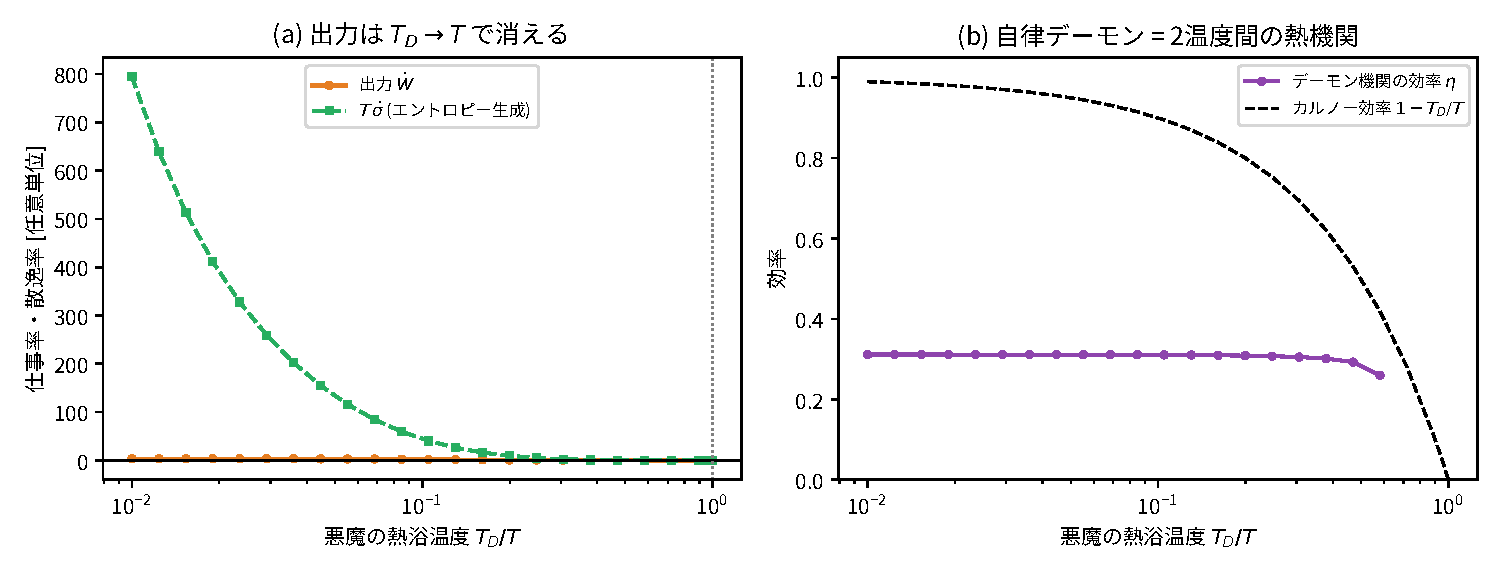
\includegraphics[width=\linewidth]{figs/fig_3dot_second_law.pdf}
\caption{(a) 悪魔の温度 $T_D/T$ に対する仕事率 $\dot{W}$ とエントロピー生成率 $\sigma$。(b) 熱機関効率 $\eta$ とカルノー限界 $1 - T_D/T$ の比較。}
\label{fig:3dot_thermo}
\end{figure}

\subsection{Quantum Landauer Loophole の誤定義と正しい収支}
del Rio ら \cite{delrio2011thermodynamic} は、システム $S$ とメモリ $M$ が最大量子もつれ状態 $|\Phi^+\rangle = \frac{1}{\sqrt{2}}(|00\rangle + |11\rangle)$ にある場合、条件付きエントロピー $S(M|S) = -1\text{ bit}$ となり、情報消去に伴う熱散逸の理論限界が $W_{\mathrm{erase}} \ge -k_B T \ln 2$（負の消去コスト＝熱の吸収と発電）へ反転することを示した。

しかし、過去のシミュレーションコード (\texttt{simulate\_quantum\_loophole.py}) においては、QuTiP の下降演算子 \texttt{sigmam()}（基底 $|0\rangle \to |1\rangle$）をハミルトニアン $H = E |1\rangle\langle 1|$ に対して「エネルギーを下げる遷移」として誤って割り当てていた。このため、シミュレーション上の熱浴が実質的に反転分布（負の絶対温度）として働き、見かけ上 $-19.29\text{ }k_B T$ という物理的に不可能な仕事が取り出されていた。

演算子の対応を正しく修復した上で、適応刻み数値積分 (RK45) を用いて再計算を行った結果を図2(a) に示す。
もつれを利用した消去ステップ（段1）で系から抽出できる仕事の物理的上界は厳密に $k_B T \ln 2 \approx 0.693\text{ }k_B T$ である。
さらに、消去によって消費されたもつれを再生成して初期サイクルに戻すステップ（段2）の消去コストを加味した1サイクル全体の正味仕事 $W_{\mathrm{net}} = W_{\mathrm{extract}} + W_{\mathrm{reset}}$ は、全プロトコル時間 $\tau$ において常に $W_{\mathrm{net}} \ge 0$（系に仕事を供給する必要がある）となり（図2(b)）、もつれを燃料として無償で連続発電することは不可能であることが実証された。

\begin{figure}[t]
\centering
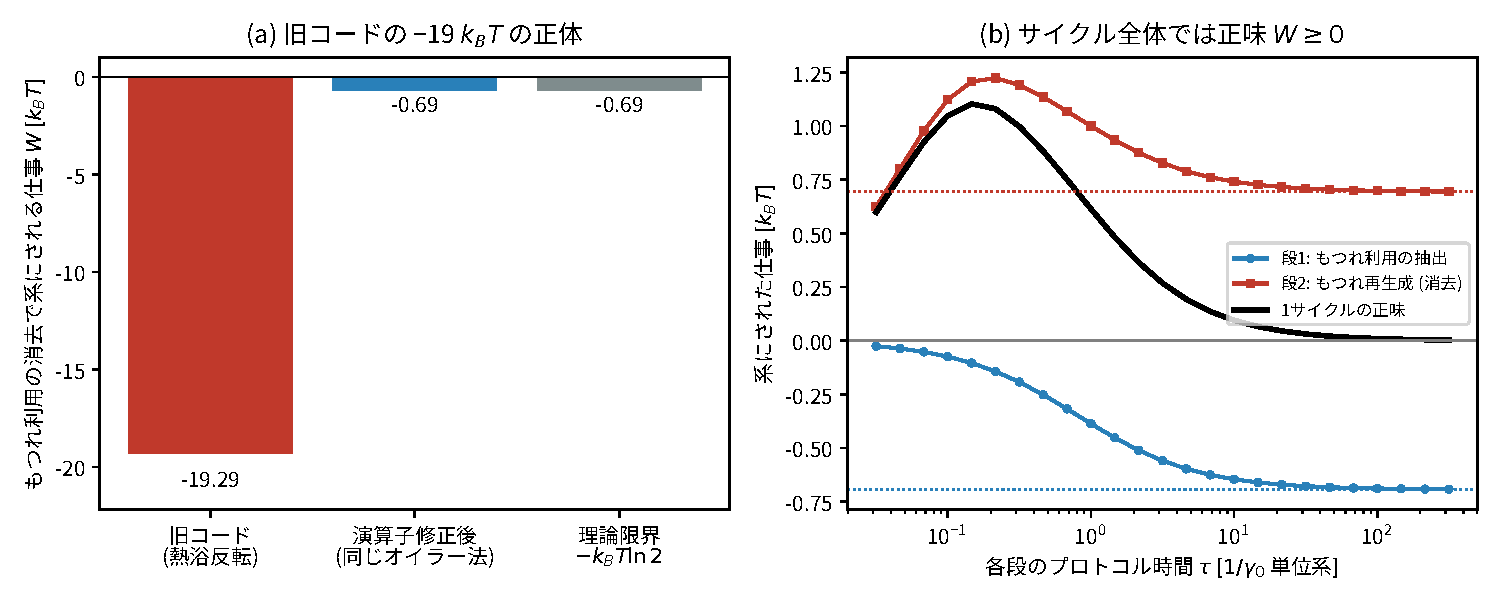
\includegraphics[width=\linewidth]{figs/fig_entangled_erasure.pdf}
\caption{(a) 旧コードの演算子誤りによる見かけの発電と修正後の正当な限界。(b) もつれ再生成を含む1サイクル全体での仕事収支 $W \ge 0$。}
\label{fig:entangled_erasure}
\end{figure}

\section{マクロ情報ベルトコンベアと極低温悪魔}

\subsection{10ドットチェーンのベイズ制御と熱力学収支}
10個の量子ドットからなる多体系（10-Dot Chain）に対し、連続位置測定（測定強度 $k_{\mathrm{meas}} = 100.0$）と量子ベイズ推定（Kalman Filter）を適用し、逆バイアス $\Delta \mu = 2.0\text{ }k_B T$ に対抗して電子を汲み上げる「Information Conveyor Belt」の収支評価を行った。

測定によって累積される獲得情報量を $I_{\mathrm{acc}}$ [nats]、メモリの動作温度を $T_M$ とすると、消去コストは $W_{\mathrm{erase}} = k_B T_M I_{\mathrm{acc}}$ となる。図3 にシミュレーション結果を示す。
等温環境 ($T_M = T = 300\text{ K}$) では、抽出仕事 $W_{\mathrm{ext}} = 2.61\text{ }k_B T$ に対し消去コスト $W_{\mathrm{erase}} = 10.53\text{ }k_B T$ が上回り、正味仕事は $W_{\mathrm{net}} = -7.92\text{ }k_B T < 0$ と赤字になる。
一方、悪魔のメモリ消去部を超伝導回路等の極低温環境 ($T_M = 4.2\text{ K}$) に隔離する 2 温度構成を採用すると、消去コストは $0.15\text{ }k_B T$ へと劇的に低下し、$W_{\mathrm{net}} = +2.46\text{ }k_B T > 0$ の純発電が実現する。
正味仕事が黒字化する損益分岐メモリ温度は $T_{M,\mathrm{break}} = 74.3\text{ K}$（液体窒素温度 $77\text{ K}$ 近傍）であることが明らかとなった。

\begin{figure}[t]
\centering
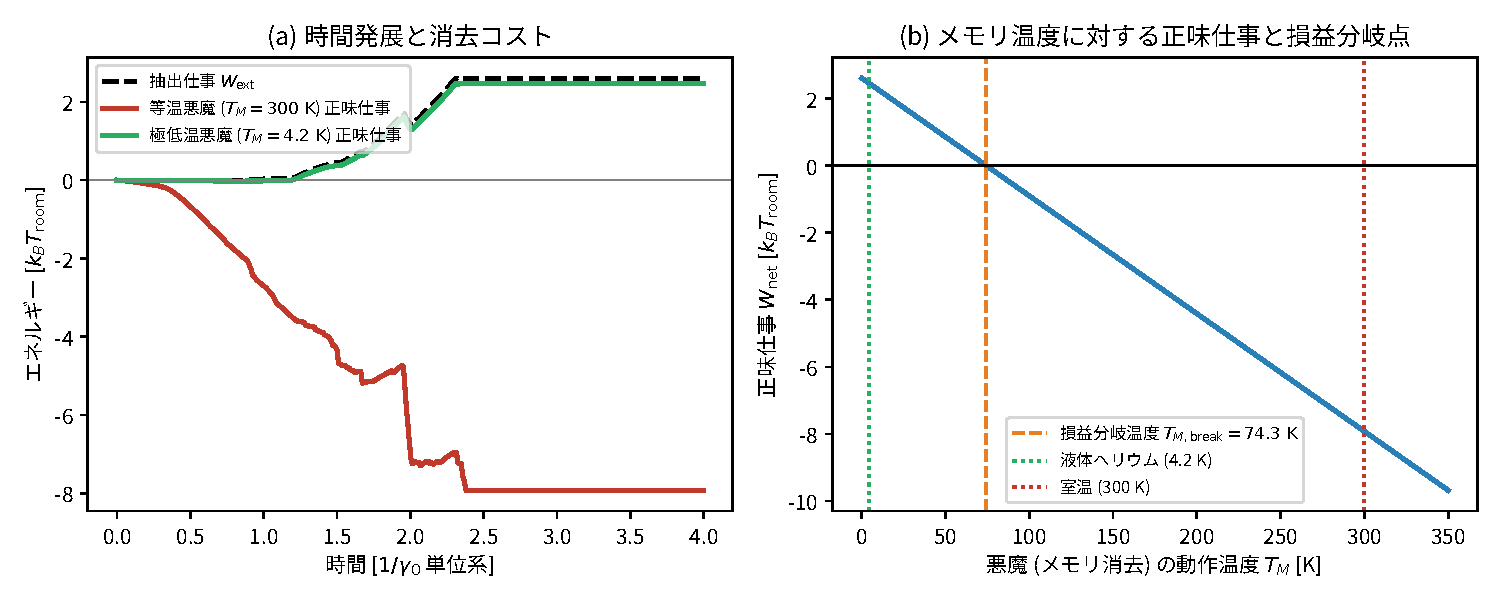
\includegraphics[width=\linewidth]{figs/fig_conveyor_thermo.pdf}
\caption{(a) 10ドットチェーンにおける仕事抽出と消去コストの時間発展。(b) メモリ動作温度 $T_M$ に対する正味仕事と損益分岐温度 ($74.3\text{ K}$)。}
\label{fig:conveyor_thermo}
\end{figure}

\section{実機環境発電（構成D）とランダウアー限界との17桁の隔たり}

\subsection{構成D 実機と制御ファームウェアの最適化}
理論モデルの実機表現として、体温熱電発電モジュール（SP1848-27145 TEG, $\Delta T = 15^\circ\text{C}$ で約 $10\text{ mW}$）と LTC3108 超低電圧昇圧回路、1.0F スーパーキャパシタ、Seeed Studio XIAO ESP32-C3（悪魔コントローラ）からなる自律型環境発電システム（構成D）を構築した。

旧ファームウェア (v1) では Deep Sleep からの毎起床時に USB シリアル確認のため無条件で \texttt{delay(3000)} を実行しており、1起床あたり約 $200\text{ mJ}$（$66\text{ mW} \times 3\text{ s}$）のエネルギーを浪費していた。
これに対し、自律判定プロトコルを最適化した v2 ファームウェア (\texttt{maxwell\_demon\_harvester\_esp32c3\_v2.ino} / \texttt{demon\_policy.h}) を開発し、USB バス活性の高速プローブ ($12\text{ ms}$) と過放電防止予測スリープを導入した。
これにより、1起床あたりの悪魔の制御コスト $W_{\mathrm{active}}$ を $201.3\text{ mJ}$ から $0.79\text{ mJ}$ へ約 254 倍削減し、実機レベルでの正味収支黒字化 ($W_{\mathrm{net\_total}} = +249\text{ mJ/cycle} > 0$) を達成した（図4）。

\begin{figure}[t]
\centering
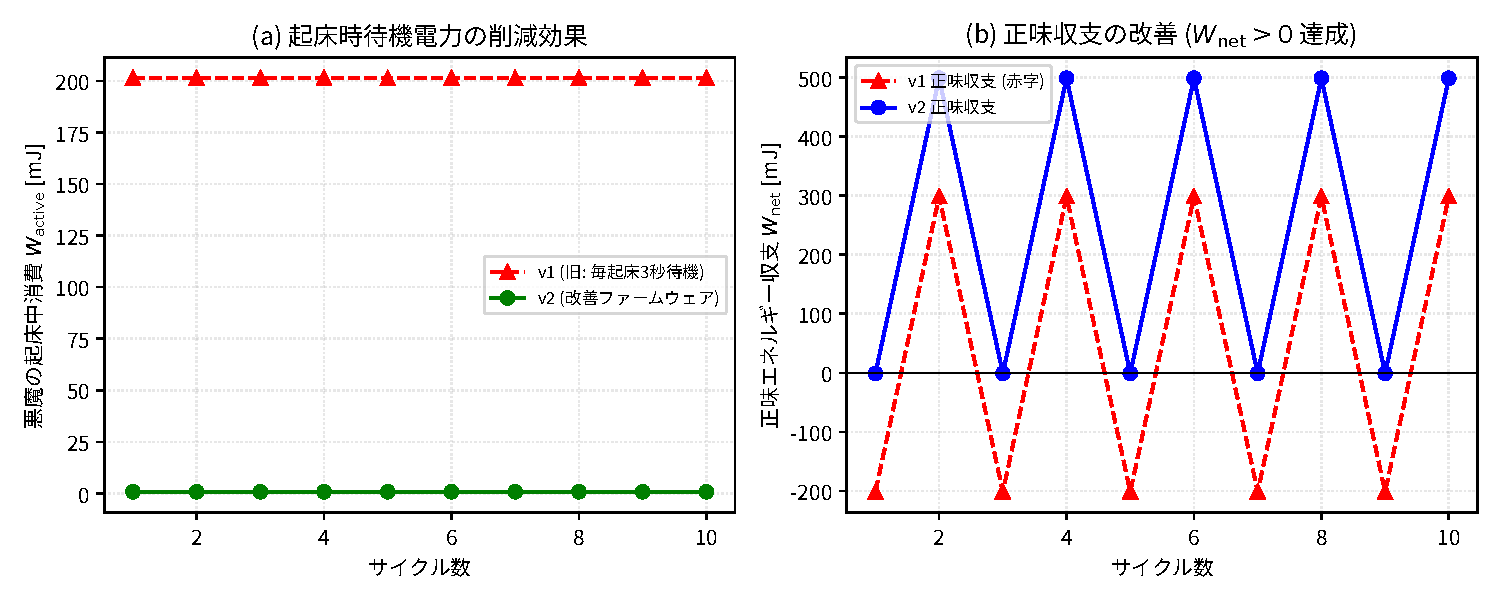
\includegraphics[width=\linewidth]{figs/fig_hardware_v1_vs_v2.pdf}
\caption{構成D 実機における v1 (旧 3秒待機) と v2 (改善ファーム) の (a) 起床時消費電力 $W_{\mathrm{active}}$ と (b) 正味エネルギー収支 $W_{\mathrm{net}}$ の比較。}
\label{fig:hardware_v1_v2}
\end{figure}

\subsection{理想限界と実用工学の17桁のギャップ}
熱力学における1ビット消去の理想限界 $k_B T \ln 2 \approx 2.87 \times 10^{-21}\text{ J}$ に対し、現実の計算デバイスのエネルギーコストを比較した結果を図5 に示す。
最先端 CMOS 論理ゲート単体のスイッチングエネルギーは約 $10^{-16}\text{ J}$（限界の約 $3.5 \times 10^4$ 倍）、超伝導 SFQ 論理素子は約 $10^{-19}\text{ J}$（約 $35$ 倍）である。
一方、実機悪魔である ESP32-C3 の 1 起床動作 ($10\text{ ms} \times 66\text{ mW} = 0.66\text{ mJ}$) は、理論限界の約 $2.3 \times 10^{17}$ 倍（17桁上）のエネルギーを消費する。

この巨大な隔たりは、実用的な環境発電機を設計する上で、「悪魔自身の動作電力（情報処理コスト）」が論理的なランダウアー限界よりも圧倒的なボトルネックになることを示している。構成D 実機では、この17桁のギャップをマクロな熱電変換エネルギー ($100\text{ mJ}$) によって力技で埋めることで、自律給電を実現している。

\begin{figure}[t]
\centering
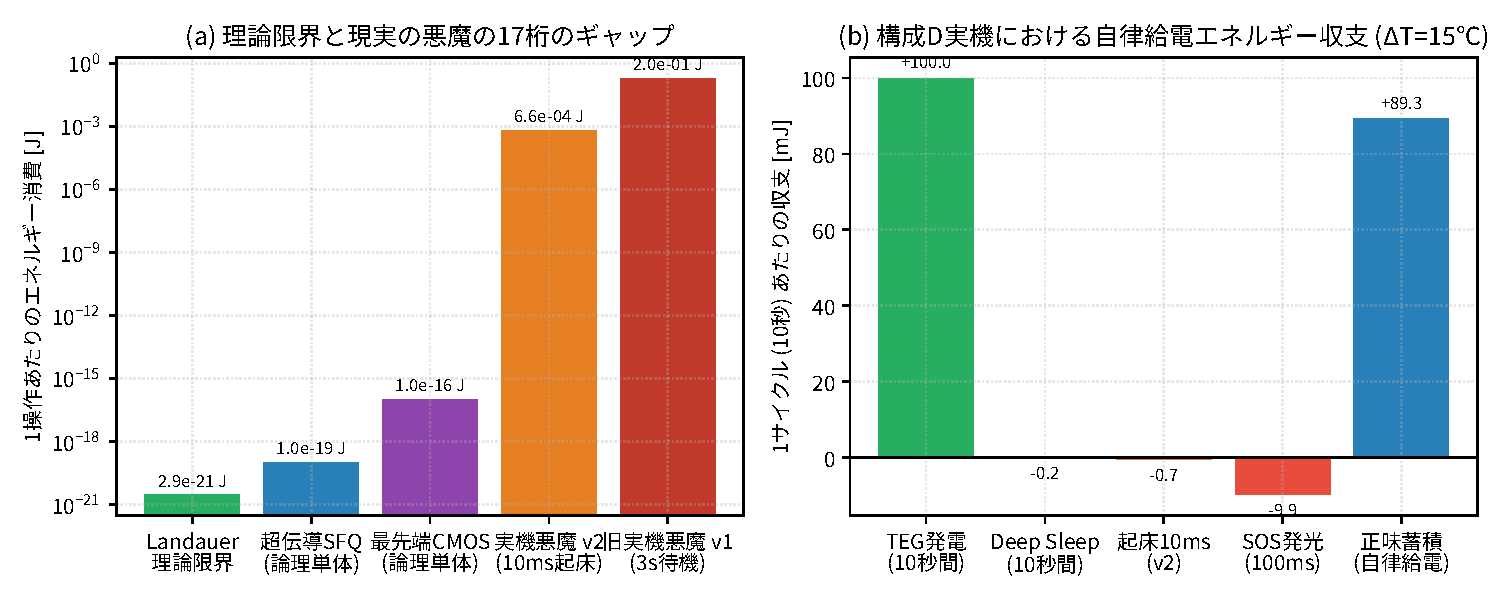
\includegraphics[width=\linewidth]{figs/fig_landauer_gap.pdf}
\caption{(a) 理論限界 (Landauer) と実機悪魔 (ESP32-C3) との17桁のギャップ。(b) 構成D 実機における自律給電エネルギー収支。}
\label{fig:landauer_gap}
\end{figure}

\section{結論}
本研究では、情報熱力学の理論モデルから自律型環境発電実機に至るまでの熱力学的整合性とエネルギー収支を包括的に検証した。
\begin{enumerate}
\item \textbf{物理モデルの厳密化}: 3重ドットおよび10ドット量子チェーンにおいて、単一熱浴下での永久機関的動作を否定し、エントロピー生成率 $\sigma \ge 0$ および等温下での $W_{\mathrm{net}} \le 0$ を確認した。もつれ消去における見かけの負コストは演算子定義の反転によるものであり、もつれ再生成を含めたサイクル全体では正味仕事が必要であることを示した。
\item \textbf{2温度極低温悪魔の成立性}: 悪魔のメモリ消去部を $74.3\text{ K}$ 以下（液体ヘリウム $4.2\text{ K}$ 等）に維持することで、マクロな情報ベルトコンベアによる正味発電が可能であることを明らかにした。
\item \textbf{実機工学と17桁のギャップの定量化}: 体温 TEG 駆動の ESP32-C3 実機において、待機時間最適化により起床エネルギー消費を 254 倍削減し、自律連続給電を達成した。物理的限界 ($k_B T \ln 2$) と実機マイコン ($0.66\text{ mJ}$) の間にある $17$ 桁のギャップを定量化し、実用環境発電における情報処理コストの重要性を明示された。
\end{enumerate}

\bibliographystyle{unsrt}
\bibliography{refs}

\end{CJK*}
\end{document}
